% ----------------------------------------------------------------------------
% Copyright (c) 2016 - 2020 by Burkhardt Renz. All rights reserved.
% Die Vorlage für eine Abschlussarbeit in der Informatik am Fachbereich
% MNI der THM ist lizenziert unter einer Creative Commons
% Namensnennung-Nicht kommerziell 4.0 International Lizenz.
%
% Id:$
% ----------------------------------------------------------------------------

\chapter{Frontend Frameworks}

In diesem Kapitel möchte ich zunächst allgemein in die JavaScript-Frontend-Frameworks einführen.
Die Drei aktuell gängigsten Frontend-Frameworks React.js, Angular und Vue.js werden vorgestellt.
\\
An eine moderne Webapplikation werden hohe Anforderungen an den Funktionsumfang durch den Benutzer gestellt.
Die Entwickler einer solchen Webapplikation erwarten eine einheitliche Codequalität und einheitliche Strukturen
für eine bessere Wartbarkeit der Webapplikation.
Um bei dem Erstellen neuer Webapplikationen den Entwickler dabei zu unterstützen diese Ziele zu erfüllen,
werden unter anderem entsprechende Frontend Frameworks verwendet.
\begin{quote}
    Front-end frameworks determine the logic, structure, design, behavior,
    and animation of every element you see on-screen when you interact with websites,
    web applications, and mobile apps. \cite{sigdestad22}
\end{quote}
Man kann zwischen UI-Frameworks in HTML und CSS sowie JavaScript-Frameworks unterscheiden.
Letztere dienen als Verbindung zwischen der Darstellung und der Logik im Frontend.

\begin{figure}[!htb]
    \centering
    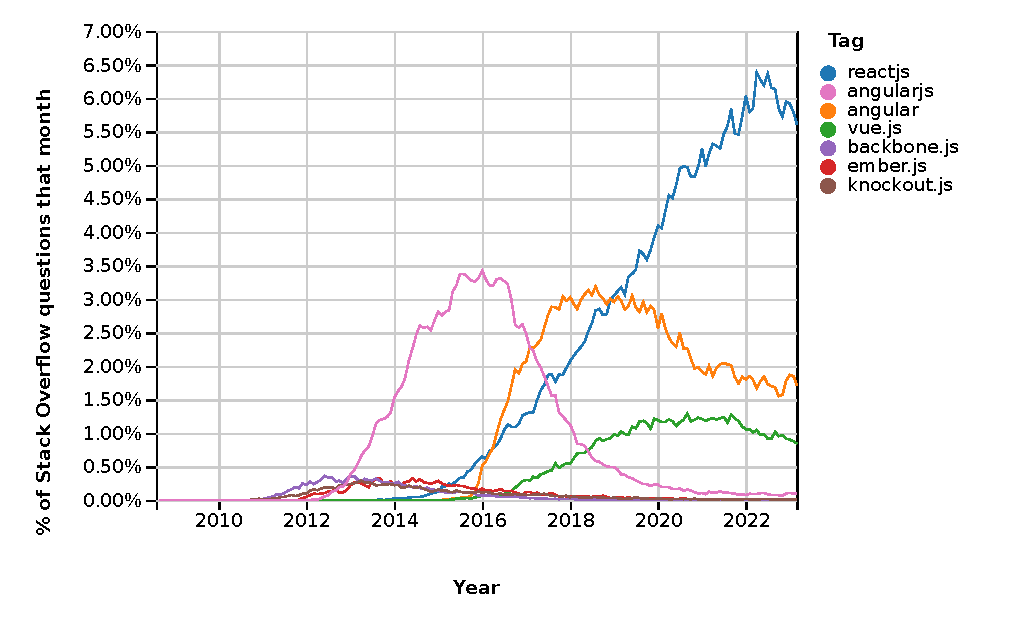
\includegraphics[width=0.8\textwidth]{img/js_frameworks_statistic_stackoverflow}
    \caption{Stackoverflow Statistik zur Häufigkeit von nach Framework}
    \label{fig:stackoverflow_stat}
\end{figure}


\begin{figure}[!htb]
    \centering
    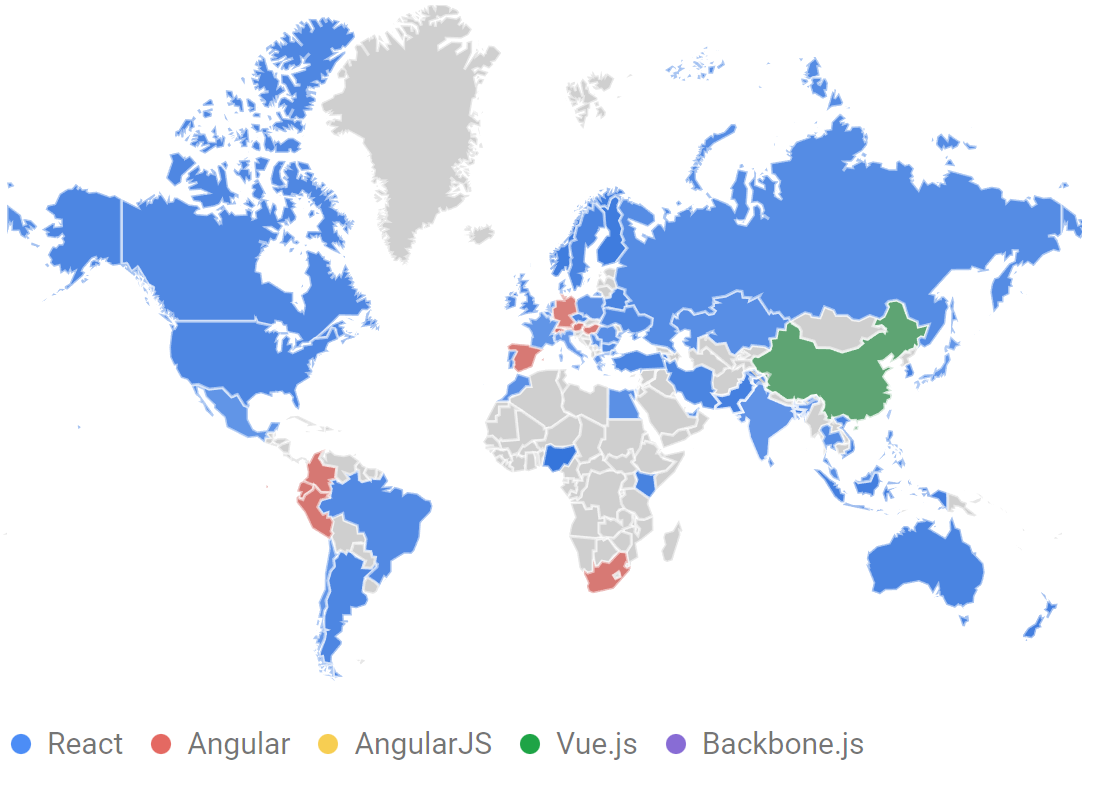
\includegraphics[width=0.8\textwidth]{img/Google Stats/2023-04-26 12_20_26-React, Angular, AngularJS, Vue.js, Backbone.js - Erkunden - Google Trends}
    \caption{Googlge Trends Weltweiteverteilung von Suchanfragen nache Framework der letzten 5 Jahre}
    \label{fig:google_trends_world}
\end{figure}

\begin{figure}[!htb]
    \centering
    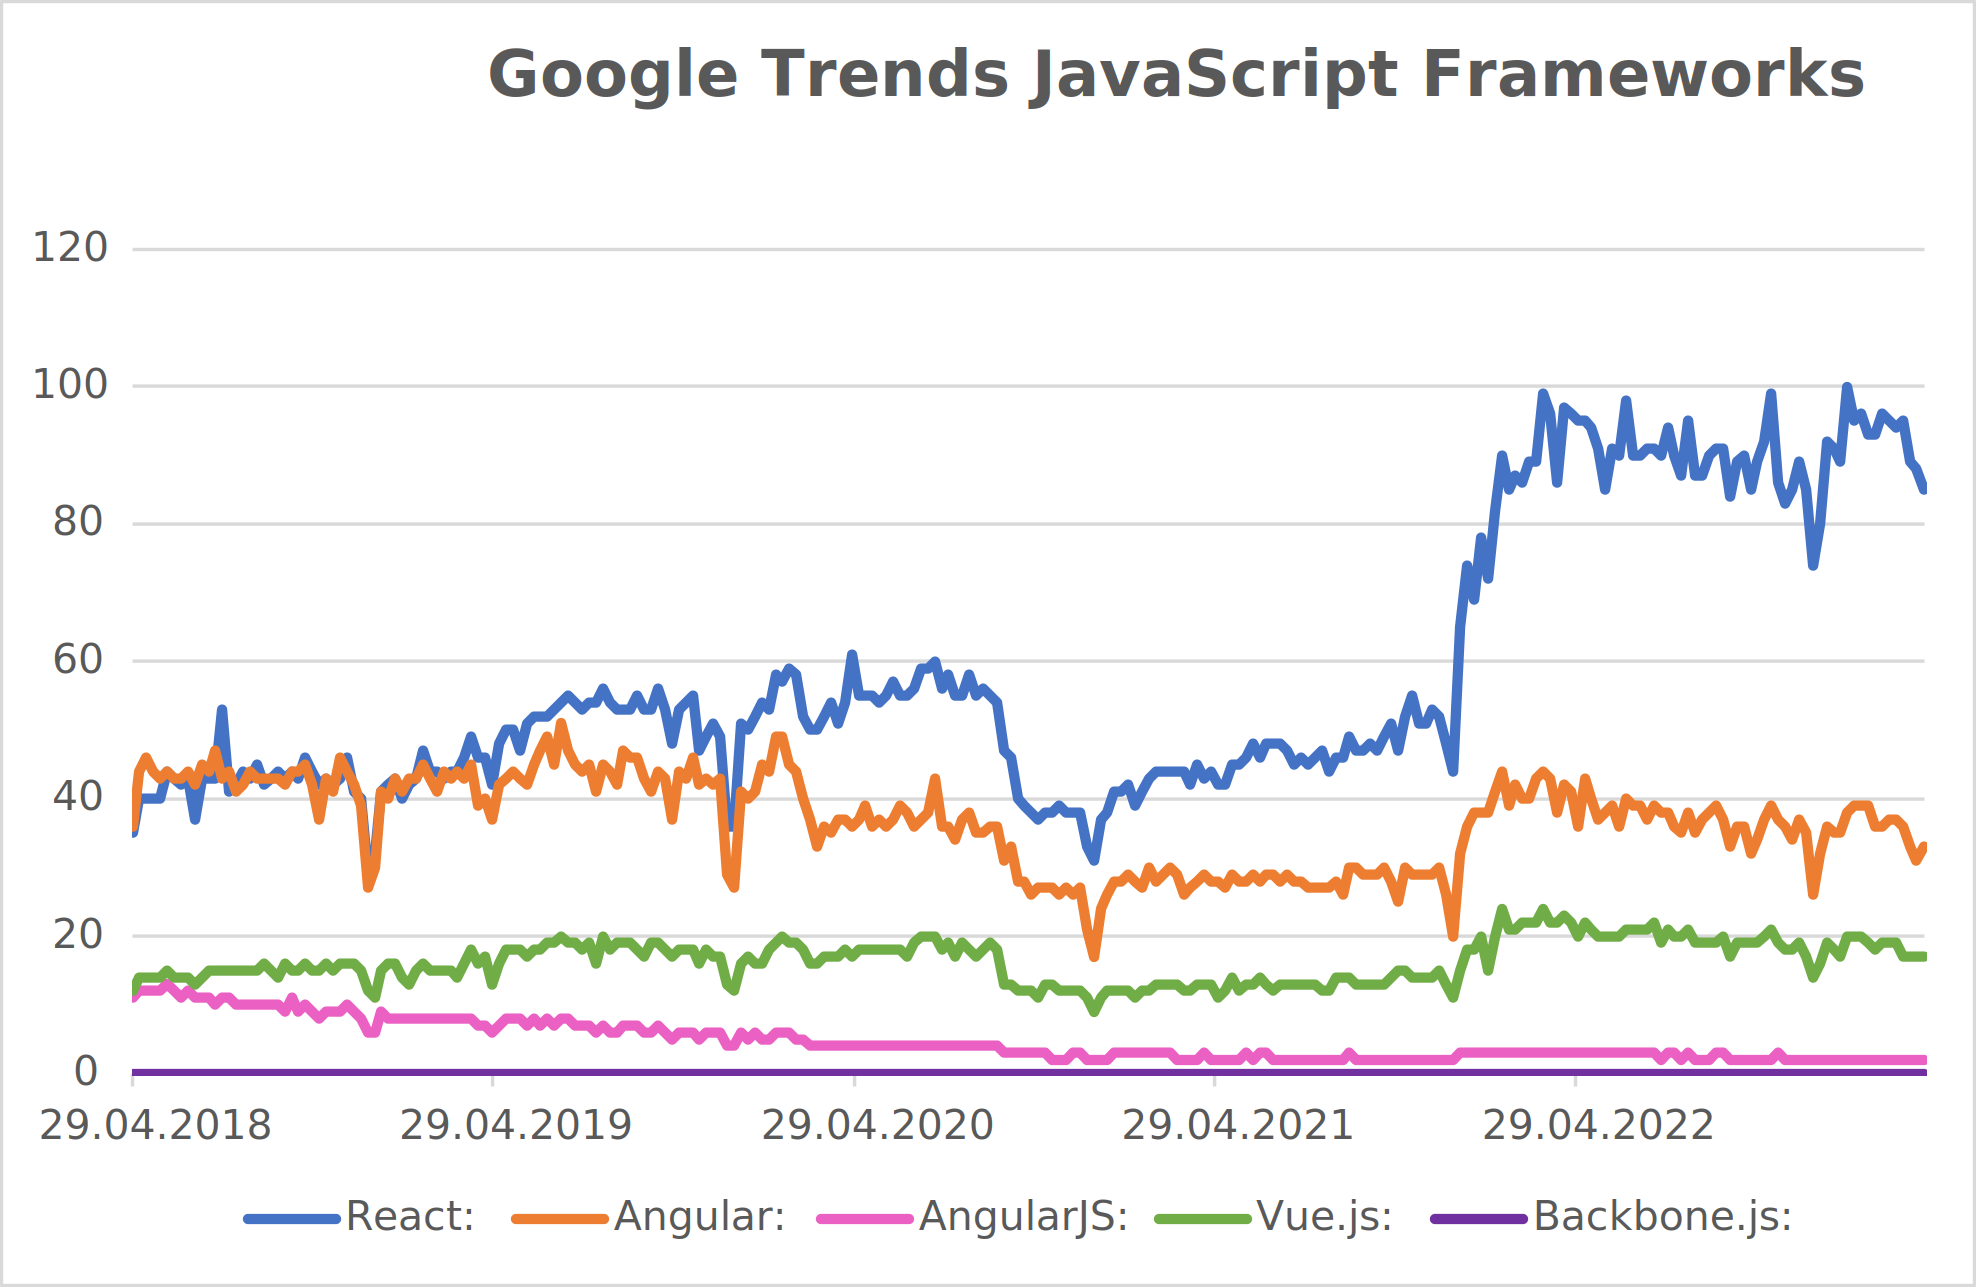
\includegraphics[width=0.8\textwidth]{img/Google Stats/google_frameworks_trends}
    \caption{Googlge Trends zur Häufigkeit von Suchanfragen nache Framework der letzten 5 Jahre}
    \label{fig:google_trends}
\end{figure}

%https://trends.google.de/trends/explore/GEO_MAP/1682502600?hl=de&tz=-120&date=today+5-y&hl=de&q=%2Fm%2F012l1vxv,%2Fg%2F11c6w0ddw9,%2Fm%2F0j45p7w,%2Fg%2F11c0vmgx5d,%2Fm%2F0h94450&sni=3
%https://insights.stackoverflow.com/trends?tags=reactjs%2Cangular%2Cvue.js%2Cember.js%2Cbackbone.js%2Cknockout.js%2Cangularjs
\section{Etwas Geschichte -- oder ein paar Geschichten}

Die ersten Bände von \emph{The Art of Computer Programming}
(\textsc{TAOCP}) von Donald Knuth wurden im Bleisatz gesetzt. In den
1970er Jahren aber starb der Bleisatz aus und wurde durch den Fotosatz
ersetzt. Knuth war mit den damaligen Fotosatz-Systemen sehr unzufrieden,
weil sie mathematische Formeln nicht gut darstellen konnten. Das brachte
ihn auf die Idee selbst ein Satzsystem zu entwickeln, das für
Texte der Mathematik und Informatik typografisch hochwertige Ergebnisse
erreichen sollte. Zunächst dachte er, ein solches Programm könne in
einem Jahr oder so erstellt werden. Es dauerte dann doch etwa
länger -- siehe Tabelle \ref{tbl:geschichte}.\footnote{ Die Entwicklung
von \TeX\ ist auch ein interessanter Fall von Software-Engineering,
    siehe Donald E. Knuth \emph{The Errors of \TeX} in: Tom de Marco und
    Timothy Lister (Hrsg.) \emph{Software State-of-the-Art: Selected
    Papers} New York NY: Dorste Publishing House, 1990.}

Knuths Idee \cite{knuth99} bestand darin, dass Text, Formeln und Layout
gewissermaßen programmiert werden. Das Satzsystem konsumiert ein solches
\enquote{Programm} und macht daraus ein Dokument --- heutzutage in der
Regel ein PDF-Dokument. Das System sollte natürlich erweiterbar und
anpassbar sein, weshalb die Sprache, die Knuth entwickelt hat, im Grunde
eine Makrosprache ist und es deshalb auch erlaubt eigene Befehle zu
schreiben. Knuth hat einen Satz an Makros entwickelt, den man
\textsc{Plain}\kern2pt\TeX\ nennt -- diese Makros sind sehr nahe am Kern
von \TeX, \emph{low level} sozusagen.

Leslie Lamport\footnote{ Leslie Lamport hat wichtige Beiträge zur
Theorie verteilter Systeme geleistet.} hat eine Menge von Makros
entwickelt, die auf \TeX\ aufbauen und das Setzen von Büchern, Berichten
und Artikeln erheblich vereinfachen. Diese Makros nannte er \LaTeX\
\cite{lamport94}. Leslie Lamport erzählt über die Entstehung von
\LaTeX\
(\url{http://research.microsoft.com/en-us/um/people/lamport/pubs/pubs.html#latex}):

\begin{quote}
    In the early 80s, I was planning to write the Great American Concurrency
    Book. I was a \TeX\ user, so I would need a set of macros. I thought
    that, with a little extra effort, I could make my macros usable by
    others. Don Knuth had begun issuing early releases of the current
    version of \TeX, and I figured I could write what would become its
    standard macro package. That was the beginning of \LaTeX.    \\
    \dots\\
    Meanwhile, I still haven't written the Great American Concurrency
    Book.
\end{quote}

\LaTeX\ trennt im Grunde die Befehle, die den Inhalt und die Struktur
eines Texts betreffen von den Befehlen, die für die typografische
Gestaltung sorgen.  \LaTeX\ stellt eine Reihe von sogenannten
Dokumentklassen bereit, die das Layout von Artikeln, Berichten, Büchern
und Briefen bereits enthalten, so dass man sich beim Schreiben nicht
mehr darum kümmern muss.

Die Dokumentklassen von \LaTeX\ erzeugen eine Typografie, die an
amerikanischen Konventionen orientiert ist. \textsf{KOMA-Script} ist eine
Sammlung von Dokumentklassen, die sich an europäischer Typografie
orientieren. Frank Neukam entwickelte Anfang der 1990er Jahr
\textsf{Script}, das Markus Kohm zu \textsf{KOMA-Script}
weiterentwickelte \cite{koma16}. Wir verwenden für die Vorlage die
Dokumentklasse von \textsf{KOMA-Script} für das Setzen von Büchern.


\section{Der Aufbau einer \LaTeX-Datei}
\label{sec:aufbau}

Eine \LaTeX-Datei beginnt mit der Angabe der Dokumentklasse mitsamt
ihren Optionen. Darauf folgt die sogenannte Präambel, in der benötigte
Pakete angegeben, Einstellungen festgelegt und auch eigene Makros
definiert werden. Darauf folgt in der Umgebung \verb=document= der
eigentliche Text.

\subsection{Dokumentklasse}

Wir verwenden für die Abschlussarbeit die Dokumentklasse \verb=scrbook=
von \textsf{KOMA-Script}. Diese Dokumentklasse ist vorgesehen für den
Satz von Büchern und sorgt dafür, dass Kapitel immer auf einer rechten
(also vorderen) Seite beginnen.

Die Dokumentklasse hat in der Regel geeignete Voreinstellungen für eine
Abschlussarbeit. Deshalb ändern wir nur einige wenige der Optionen von
\verb=scrbook=. In \cite{partosch15} werden weitere Optionen erläutert.

\subsection{Präambel}

In der Präambel binden wir benötigte Pakete ein. Pakete sind
vorgefertigte Sammlungen von Makros für \LaTeX. Es gibt für nahezu jede
denkbare Aufgabe solche Pakete, die man im \TeX\ Catalogue
\url{http://texcatalogue.ctan.org} finden kann.

Unsere Vorlage bindet die wichtigsten und für eine Arbeit im Feld der
Informatik in der Regel benötigten Pakete ein. Auch hierzu findet man
weitere Informationen in \cite{partosch15}.

Darüber hinaus stehen Einstellungen in der Präambel, bei uns z.B. zur
Nummerierungstiefe.

Eigene Makros kann man auch in der Präambel unterbringen.

\subsection{Die Umgebung \texttt{document}}

Nach der Präambel kommt die Umgebung \verb=document=. In \LaTeX\ nennt
man Blöcke, die durch \verb=\begin{umgebung}= und \verb=\end{umgebung}=
begrenzt sind \emph{Umgebung}. In der Regel werden zu Beginn der
Umgebung bestimmte Einstellungen ein- und am Ende der Umgebung wieder
ausgeschaltet.

Der eigentliche Text der Arbeit steht also in der Klammer

\begin{lstlisting}
\begin{document}

% hierher kommt der eigentliche Text

\end{document}
\end{lstlisting}


Es ist ratsam, den eigentlichen Text in verschiedene Dateien zu
verteilen, etwa pro Kapitel eine Datei. Diese Dateien können dann in die
führende Datei eingebunden werden, bei uns durch folgende Befehle:

\begin{lstlisting}

% ----------------------------------------------------------------------------
% Copyright (c) 2016 - 2020 by Burkhardt Renz. All rights reserved.
% Die Vorlage für eine Abschlussarbeit in der Informatik am Fachbereich
% MNI der THM ist lizenziert unter einer Creative Commons
% Namensnennung-Nicht kommerziell 4.0 International Lizenz.
%
% Id:$
% ----------------------------------------------------------------------------

\chapter{Was ist \LaTeX\ und wie ist eine \LaTeX-Datei aufgebaut?}

Der Text dieses Kapitals steht in der Datei \verb=aufbau.tex=. Die
Erläuterungen ab Abschnitt \ref{sec:aufbau} beziehen sich auf die Datei
\verb=vorlage.tex=.

\section{Etwas Geschichte -- oder ein paar Geschichten}

Die ersten Bände von \emph{The Art of Computer Programming}
(\textsc{TAOCP}) von Donald Knuth wurden im Bleisatz gesetzt. In den
1970er Jahren aber starb der Bleisatz aus und wurde durch den Fotosatz
ersetzt. Knuth war mit den damaligen Fotosatz-Systemen sehr unzufrieden,
weil sie mathematische Formeln nicht gut darstellen konnten. Das brachte
ihn auf die Idee selbst ein Satzsystem zu entwickeln, das für
Texte der Mathematik und Informatik typografisch hochwertige Ergebnisse
erreichen sollte. Zunächst dachte er, ein solches Programm könne in
einem Jahr oder so erstellt werden. Es dauerte dann doch etwa
länger -- siehe Tabelle \ref{tbl:geschichte}.\footnote{ Die Entwicklung
von \TeX\ ist auch ein interessanter Fall von Software-Engineering,
siehe Donald E. Knuth \emph{The Errors of \TeX} in: Tom de Marco und
Timothy Lister (Hrsg.) \emph{Software State-of-the-Art: Selected
Papers} New York NY: Dorste Publishing House, 1990.}

Knuths Idee \cite{knuth99} bestand darin, dass Text, Formeln und Layout
gewissermaßen programmiert werden. Das Satzsystem konsumiert ein solches
\enquote{Programm} und macht daraus ein Dokument --- heutzutage in der
Regel ein PDF-Dokument. Das System sollte natürlich erweiterbar und
anpassbar sein, weshalb die Sprache, die Knuth entwickelt hat, im Grunde
eine Makrosprache ist und es deshalb auch erlaubt eigene Befehle zu
schreiben. Knuth hat einen Satz an Makros entwickelt, den man
\textsc{Plain}\kern2pt\TeX\ nennt -- diese Makros sind sehr nahe am Kern
von \TeX, \emph{low level} sozusagen.

Leslie Lamport\footnote{ Leslie Lamport hat wichtige Beiträge zur
Theorie verteilter Systeme geleistet.} hat eine Menge von Makros
entwickelt, die auf \TeX\ aufbauen und das Setzen von Büchern, Berichten
und Artikeln erheblich vereinfachen. Diese Makros nannte er \LaTeX\
\cite{lamport94}.  Leslie Lamport erzählt über die Entstehung  von
\LaTeX\
(\url{http://research.microsoft.com/en-us/um/people/lamport/pubs/pubs.html#latex}):

\begin{quote}
In the early 80s, I was planning to write the Great American Concurrency
Book.  I was a \TeX\ user, so I would need a set of macros.  I thought
that, with a little extra effort, I could make my macros usable by
others.  Don Knuth had begun issuing early releases of the current
version of \TeX, and I figured I could write what would become its
standard macro package.  That was the beginning of \LaTeX. 	\\
\dots\\
Meanwhile, I still haven't written the Great American Concurrency
Book.
\end{quote}

\LaTeX\ trennt im Grunde die Befehle, die den Inhalt und die Struktur
eines Texts betreffen von den Befehlen, die für die typografische
Gestaltung sorgen.  \LaTeX\ stellt eine Reihe von sogenannten
Dokumentklassen bereit, die das Layout von Artikeln, Berichten, Büchern
und Briefen bereits enthalten, so dass man sich beim Schreiben nicht
mehr darum kümmern muss.

Die Dokumentklassen von \LaTeX\ erzeugen eine Typografie, die an
amerikanischen Konventionen orientiert ist. \textsf{KOMA-Script} ist eine
Sammlung von Dokumentklassen, die sich an europäischer Typografie
orientieren. Frank Neukam entwickelte Anfang der 1990er Jahr
\textsf{Script}, das Markus Kohm zu \textsf{KOMA-Script}
weiterentwickelte \cite{koma16}. Wir verwenden für die Vorlage die
Dokumentklasse von \textsf{KOMA-Script} für das Setzen von Büchern.

\section{Der Aufbau einer \LaTeX-Datei}
\label{sec:aufbau}

Eine \LaTeX-Datei beginnt mit der Angabe der Dokumentklasse mitsamt
ihren Optionen. Darauf folgt die sogenannte Präambel, in der benötigte
Pakete angegeben, Einstellungen festgelegt und auch eigene Makros
definiert werden. Darauf folgt in der Umgebung \verb=document= der
eigentliche Text.

\subsection{Dokumentklasse}

Wir verwenden für die Abschlussarbeit die Dokumentklasse \verb=scrbook=
von \textsf{KOMA-Script}. Diese Dokumentklasse ist vorgesehen für den
Satz von Büchern und sorgt dafür, dass Kapitel immer auf einer rechten
(also vorderen) Seite beginnen.

Die Dokumentklasse hat in der Regel geeignete Voreinstellungen für eine
Abschlussarbeit. Deshalb ändern wir nur einige wenige der Optionen von
\verb=scrbook=. In \cite{partosch15} werden weitere Optionen erläutert.

\subsection{Präambel}

In der Präambel binden wir benötigte Pakete ein.  Pakete sind
vorgefertigte Sammlungen von Makros für \LaTeX. Es  gibt für nahezu jede
denkbare Aufgabe solche Pakete, die man im \TeX\ Catalogue
\url{http://texcatalogue.ctan.org} finden kann.

Unsere Vorlage bindet die wichtigsten und für eine Arbeit im Feld der
Informatik in der Regel benötigten Pakete ein. Auch hierzu findet man
weitere Informationen in \cite{partosch15}.

Darüber hinaus stehen Einstellungen in der Präambel, bei uns z.B. zur
Nummerierungstiefe.

Eigene Makros kann man auch in der Präambel unterbringen.

\subsection{Die Umgebung \texttt{document}}

Nach der Präambel kommt die Umgebung \verb=document=. In \LaTeX\ nennt
man Blöcke, die durch \verb=\begin{umgebung}= und \verb=\end{umgebung}=
begrenzt sind \emph{Umgebung}. In der Regel werden zu Beginn der
Umgebung bestimmte Einstellungen ein- und am Ende der Umgebung wieder
ausgeschaltet.

Der eigentliche Text der Arbeit steht also in der Klammer

\begin{lstlisting}
\begin{document}

% hierher kommt der eigentliche Text

\end{document}
\end{lstlisting}


Es ist ratsam, den eigentlichen Text in verschiedene Dateien zu
verteilen, etwa pro Kapitel eine Datei. Diese Dateien können dann in die
führende Datei eingebunden werden, bei uns durch folgende Befehle:

\begin{lstlisting}

% ----------------------------------------------------------------------------
% Copyright (c) 2016 - 2020 by Burkhardt Renz. All rights reserved.
% Die Vorlage für eine Abschlussarbeit in der Informatik am Fachbereich
% MNI der THM ist lizenziert unter einer Creative Commons
% Namensnennung-Nicht kommerziell 4.0 International Lizenz.
%
% Id:$
% ----------------------------------------------------------------------------

\chapter{Was ist \LaTeX\ und wie ist eine \LaTeX-Datei aufgebaut?}

Der Text dieses Kapitals steht in der Datei \verb=aufbau.tex=. Die
Erläuterungen ab Abschnitt \ref{sec:aufbau} beziehen sich auf die Datei
\verb=vorlage.tex=.

\section{Etwas Geschichte -- oder ein paar Geschichten}

Die ersten Bände von \emph{The Art of Computer Programming}
(\textsc{TAOCP}) von Donald Knuth wurden im Bleisatz gesetzt. In den
1970er Jahren aber starb der Bleisatz aus und wurde durch den Fotosatz
ersetzt. Knuth war mit den damaligen Fotosatz-Systemen sehr unzufrieden,
weil sie mathematische Formeln nicht gut darstellen konnten. Das brachte
ihn auf die Idee selbst ein Satzsystem zu entwickeln, das für
Texte der Mathematik und Informatik typografisch hochwertige Ergebnisse
erreichen sollte. Zunächst dachte er, ein solches Programm könne in
einem Jahr oder so erstellt werden. Es dauerte dann doch etwa
länger -- siehe Tabelle \ref{tbl:geschichte}.\footnote{ Die Entwicklung
von \TeX\ ist auch ein interessanter Fall von Software-Engineering,
siehe Donald E. Knuth \emph{The Errors of \TeX} in: Tom de Marco und
Timothy Lister (Hrsg.) \emph{Software State-of-the-Art: Selected
Papers} New York NY: Dorste Publishing House, 1990.}

Knuths Idee \cite{knuth99} bestand darin, dass Text, Formeln und Layout
gewissermaßen programmiert werden. Das Satzsystem konsumiert ein solches
\enquote{Programm} und macht daraus ein Dokument --- heutzutage in der
Regel ein PDF-Dokument. Das System sollte natürlich erweiterbar und
anpassbar sein, weshalb die Sprache, die Knuth entwickelt hat, im Grunde
eine Makrosprache ist und es deshalb auch erlaubt eigene Befehle zu
schreiben. Knuth hat einen Satz an Makros entwickelt, den man
\textsc{Plain}\kern2pt\TeX\ nennt -- diese Makros sind sehr nahe am Kern
von \TeX, \emph{low level} sozusagen.

Leslie Lamport\footnote{ Leslie Lamport hat wichtige Beiträge zur
Theorie verteilter Systeme geleistet.} hat eine Menge von Makros
entwickelt, die auf \TeX\ aufbauen und das Setzen von Büchern, Berichten
und Artikeln erheblich vereinfachen. Diese Makros nannte er \LaTeX\
\cite{lamport94}.  Leslie Lamport erzählt über die Entstehung  von
\LaTeX\
(\url{http://research.microsoft.com/en-us/um/people/lamport/pubs/pubs.html#latex}):

\begin{quote}
In the early 80s, I was planning to write the Great American Concurrency
Book.  I was a \TeX\ user, so I would need a set of macros.  I thought
that, with a little extra effort, I could make my macros usable by
others.  Don Knuth had begun issuing early releases of the current
version of \TeX, and I figured I could write what would become its
standard macro package.  That was the beginning of \LaTeX. 	\\
\dots\\
Meanwhile, I still haven't written the Great American Concurrency
Book.
\end{quote}

\LaTeX\ trennt im Grunde die Befehle, die den Inhalt und die Struktur
eines Texts betreffen von den Befehlen, die für die typografische
Gestaltung sorgen.  \LaTeX\ stellt eine Reihe von sogenannten
Dokumentklassen bereit, die das Layout von Artikeln, Berichten, Büchern
und Briefen bereits enthalten, so dass man sich beim Schreiben nicht
mehr darum kümmern muss.

Die Dokumentklassen von \LaTeX\ erzeugen eine Typografie, die an
amerikanischen Konventionen orientiert ist. \textsf{KOMA-Script} ist eine
Sammlung von Dokumentklassen, die sich an europäischer Typografie
orientieren. Frank Neukam entwickelte Anfang der 1990er Jahr
\textsf{Script}, das Markus Kohm zu \textsf{KOMA-Script}
weiterentwickelte \cite{koma16}. Wir verwenden für die Vorlage die
Dokumentklasse von \textsf{KOMA-Script} für das Setzen von Büchern.

\section{Der Aufbau einer \LaTeX-Datei}
\label{sec:aufbau}

Eine \LaTeX-Datei beginnt mit der Angabe der Dokumentklasse mitsamt
ihren Optionen. Darauf folgt die sogenannte Präambel, in der benötigte
Pakete angegeben, Einstellungen festgelegt und auch eigene Makros
definiert werden. Darauf folgt in der Umgebung \verb=document= der
eigentliche Text.

\subsection{Dokumentklasse}

Wir verwenden für die Abschlussarbeit die Dokumentklasse \verb=scrbook=
von \textsf{KOMA-Script}. Diese Dokumentklasse ist vorgesehen für den
Satz von Büchern und sorgt dafür, dass Kapitel immer auf einer rechten
(also vorderen) Seite beginnen.

Die Dokumentklasse hat in der Regel geeignete Voreinstellungen für eine
Abschlussarbeit. Deshalb ändern wir nur einige wenige der Optionen von
\verb=scrbook=. In \cite{partosch15} werden weitere Optionen erläutert.

\subsection{Präambel}

In der Präambel binden wir benötigte Pakete ein.  Pakete sind
vorgefertigte Sammlungen von Makros für \LaTeX. Es  gibt für nahezu jede
denkbare Aufgabe solche Pakete, die man im \TeX\ Catalogue
\url{http://texcatalogue.ctan.org} finden kann.

Unsere Vorlage bindet die wichtigsten und für eine Arbeit im Feld der
Informatik in der Regel benötigten Pakete ein. Auch hierzu findet man
weitere Informationen in \cite{partosch15}.

Darüber hinaus stehen Einstellungen in der Präambel, bei uns z.B. zur
Nummerierungstiefe.

Eigene Makros kann man auch in der Präambel unterbringen.

\subsection{Die Umgebung \texttt{document}}

Nach der Präambel kommt die Umgebung \verb=document=. In \LaTeX\ nennt
man Blöcke, die durch \verb=\begin{umgebung}= und \verb=\end{umgebung}=
begrenzt sind \emph{Umgebung}. In der Regel werden zu Beginn der
Umgebung bestimmte Einstellungen ein- und am Ende der Umgebung wieder
ausgeschaltet.

Der eigentliche Text der Arbeit steht also in der Klammer

\begin{lstlisting}
\begin{document}

% hierher kommt der eigentliche Text

\end{document}
\end{lstlisting}


Es ist ratsam, den eigentlichen Text in verschiedene Dateien zu
verteilen, etwa pro Kapitel eine Datei. Diese Dateien können dann in die
führende Datei eingebunden werden, bei uns durch folgende Befehle:

\begin{lstlisting}

% ----------------------------------------------------------------------------
% Copyright (c) 2016 - 2020 by Burkhardt Renz. All rights reserved.
% Die Vorlage für eine Abschlussarbeit in der Informatik am Fachbereich
% MNI der THM ist lizenziert unter einer Creative Commons
% Namensnennung-Nicht kommerziell 4.0 International Lizenz.
%
% Id:$
% ----------------------------------------------------------------------------

\chapter{Was ist \LaTeX\ und wie ist eine \LaTeX-Datei aufgebaut?}

Der Text dieses Kapitals steht in der Datei \verb=aufbau.tex=. Die
Erläuterungen ab Abschnitt \ref{sec:aufbau} beziehen sich auf die Datei
\verb=vorlage.tex=.

\section{Etwas Geschichte -- oder ein paar Geschichten}

Die ersten Bände von \emph{The Art of Computer Programming}
(\textsc{TAOCP}) von Donald Knuth wurden im Bleisatz gesetzt. In den
1970er Jahren aber starb der Bleisatz aus und wurde durch den Fotosatz
ersetzt. Knuth war mit den damaligen Fotosatz-Systemen sehr unzufrieden,
weil sie mathematische Formeln nicht gut darstellen konnten. Das brachte
ihn auf die Idee selbst ein Satzsystem zu entwickeln, das für
Texte der Mathematik und Informatik typografisch hochwertige Ergebnisse
erreichen sollte. Zunächst dachte er, ein solches Programm könne in
einem Jahr oder so erstellt werden. Es dauerte dann doch etwa
länger -- siehe Tabelle \ref{tbl:geschichte}.\footnote{ Die Entwicklung
von \TeX\ ist auch ein interessanter Fall von Software-Engineering,
siehe Donald E. Knuth \emph{The Errors of \TeX} in: Tom de Marco und
Timothy Lister (Hrsg.) \emph{Software State-of-the-Art: Selected
Papers} New York NY: Dorste Publishing House, 1990.}

Knuths Idee \cite{knuth99} bestand darin, dass Text, Formeln und Layout
gewissermaßen programmiert werden. Das Satzsystem konsumiert ein solches
\enquote{Programm} und macht daraus ein Dokument --- heutzutage in der
Regel ein PDF-Dokument. Das System sollte natürlich erweiterbar und
anpassbar sein, weshalb die Sprache, die Knuth entwickelt hat, im Grunde
eine Makrosprache ist und es deshalb auch erlaubt eigene Befehle zu
schreiben. Knuth hat einen Satz an Makros entwickelt, den man
\textsc{Plain}\kern2pt\TeX\ nennt -- diese Makros sind sehr nahe am Kern
von \TeX, \emph{low level} sozusagen.

Leslie Lamport\footnote{ Leslie Lamport hat wichtige Beiträge zur
Theorie verteilter Systeme geleistet.} hat eine Menge von Makros
entwickelt, die auf \TeX\ aufbauen und das Setzen von Büchern, Berichten
und Artikeln erheblich vereinfachen. Diese Makros nannte er \LaTeX\
\cite{lamport94}.  Leslie Lamport erzählt über die Entstehung  von
\LaTeX\
(\url{http://research.microsoft.com/en-us/um/people/lamport/pubs/pubs.html#latex}):

\begin{quote}
In the early 80s, I was planning to write the Great American Concurrency
Book.  I was a \TeX\ user, so I would need a set of macros.  I thought
that, with a little extra effort, I could make my macros usable by
others.  Don Knuth had begun issuing early releases of the current
version of \TeX, and I figured I could write what would become its
standard macro package.  That was the beginning of \LaTeX. 	\\
\dots\\
Meanwhile, I still haven't written the Great American Concurrency
Book.
\end{quote}

\LaTeX\ trennt im Grunde die Befehle, die den Inhalt und die Struktur
eines Texts betreffen von den Befehlen, die für die typografische
Gestaltung sorgen.  \LaTeX\ stellt eine Reihe von sogenannten
Dokumentklassen bereit, die das Layout von Artikeln, Berichten, Büchern
und Briefen bereits enthalten, so dass man sich beim Schreiben nicht
mehr darum kümmern muss.

Die Dokumentklassen von \LaTeX\ erzeugen eine Typografie, die an
amerikanischen Konventionen orientiert ist. \textsf{KOMA-Script} ist eine
Sammlung von Dokumentklassen, die sich an europäischer Typografie
orientieren. Frank Neukam entwickelte Anfang der 1990er Jahr
\textsf{Script}, das Markus Kohm zu \textsf{KOMA-Script}
weiterentwickelte \cite{koma16}. Wir verwenden für die Vorlage die
Dokumentklasse von \textsf{KOMA-Script} für das Setzen von Büchern.

\section{Der Aufbau einer \LaTeX-Datei}
\label{sec:aufbau}

Eine \LaTeX-Datei beginnt mit der Angabe der Dokumentklasse mitsamt
ihren Optionen. Darauf folgt die sogenannte Präambel, in der benötigte
Pakete angegeben, Einstellungen festgelegt und auch eigene Makros
definiert werden. Darauf folgt in der Umgebung \verb=document= der
eigentliche Text.

\subsection{Dokumentklasse}

Wir verwenden für die Abschlussarbeit die Dokumentklasse \verb=scrbook=
von \textsf{KOMA-Script}. Diese Dokumentklasse ist vorgesehen für den
Satz von Büchern und sorgt dafür, dass Kapitel immer auf einer rechten
(also vorderen) Seite beginnen.

Die Dokumentklasse hat in der Regel geeignete Voreinstellungen für eine
Abschlussarbeit. Deshalb ändern wir nur einige wenige der Optionen von
\verb=scrbook=. In \cite{partosch15} werden weitere Optionen erläutert.

\subsection{Präambel}

In der Präambel binden wir benötigte Pakete ein.  Pakete sind
vorgefertigte Sammlungen von Makros für \LaTeX. Es  gibt für nahezu jede
denkbare Aufgabe solche Pakete, die man im \TeX\ Catalogue
\url{http://texcatalogue.ctan.org} finden kann.

Unsere Vorlage bindet die wichtigsten und für eine Arbeit im Feld der
Informatik in der Regel benötigten Pakete ein. Auch hierzu findet man
weitere Informationen in \cite{partosch15}.

Darüber hinaus stehen Einstellungen in der Präambel, bei uns z.B. zur
Nummerierungstiefe.

Eigene Makros kann man auch in der Präambel unterbringen.

\subsection{Die Umgebung \texttt{document}}

Nach der Präambel kommt die Umgebung \verb=document=. In \LaTeX\ nennt
man Blöcke, die durch \verb=\begin{umgebung}= und \verb=\end{umgebung}=
begrenzt sind \emph{Umgebung}. In der Regel werden zu Beginn der
Umgebung bestimmte Einstellungen ein- und am Ende der Umgebung wieder
ausgeschaltet.

Der eigentliche Text der Arbeit steht also in der Klammer

\begin{lstlisting}
\begin{document}

% hierher kommt der eigentliche Text

\end{document}
\end{lstlisting}


Es ist ratsam, den eigentlichen Text in verschiedene Dateien zu
verteilen, etwa pro Kapitel eine Datei. Diese Dateien können dann in die
führende Datei eingebunden werden, bei uns durch folgende Befehle:

\begin{lstlisting}

\input{aufbau}      % Kapitel 1
\input{gliederung}  % Kapitel 2
\input{elemente}    % Kapitel 3

\end{lstlisting}

% ----------------------------------------------------------------------------
      % Kapitel 1
% ----------------------------------------------------------------------------
% Copyright (c) 2016 -2020 by Burkhardt Renz. All rights reserved.
% Die Vorlage für eine Abschlussarbeit in der Informatik am Fachbereich
% MNI der THM ist lizenziert unter einer Creative Commons
% Namensnennung-Nicht kommerziell 4.0 International Lizenz.
%
% Id:$
% ----------------------------------------------------------------------------

\chapter{Elemente für die Gliederung}

Der Text dieses Kapitels steht in \verb=gliederung.tex=. Er bezieht sich
auf \verb=vorlage.tex= und \verb=gliederung.tex=.

\section{Teile}

Eine Abschlussarbeit besteht aus drei großen Teilen:

\begin{itemize}
	\item Dem Vorderteil (\verb=frontmatter=) mit
		\begin{itemize}
			\item der Titelseite,
			\item der eidesstattlichen Erklärung,
			\item der Zusammenfassung,
			\item dem Inhaltsverzeichnis und
			\item den Verzeichnissen von Abbildungen, Tabellen und Listings,
		\end{itemize}
	\item dem Hauptteil (\verb=mainmatter=) mit den Kapiteln der Arbeit
		und
	\item dem Anhang (\verb=backmatter=) mit Anhängen und dem
		Literaturverzeichnis	
\end{itemize}

Manchmal erwarten Dozentinnen oder Dozenten, dass eine Abschlussarbeit
Verzeichnisse der Abbildungen, Tabellen und Listings oder auch ein Glossar
der verwendeten Begriffe enthält. Deshalb enthält unsere Vorlage diese
Verzeichnisse. Ein Glossar kann man mit der Umgebung \verb=description=
oder \verb=labeling= erzeugen, die in Abschnitt
\ref{sec:stichwortlisten}  beschrieben werden.

Ich persönlich finde, dass man auf diese Verzeichnisse verzichten kann.
Und ein Glossar ist meines Erachtens nur nötig, wenn man viele
Fachbegriffe in der Arbeit verwendet, die einem in der Informatik
Kundigen nicht geläufig sind.

\section{Kapitel und ihre Untergliederungen}

Die Dokumentklasse \verb=scrbook= hat als Möglichkeiten der Gliederung
zunächst den Teil (\verb=part=). Er wird in diesem Dokument nicht
verwendet und meistens ist eine Bachelor- oder Masterarbeit nicht so
umfangreich, als dass man sie in Teile unterteilen müsste.

Die nächste Ebene ist das Kapital (\verb=chapter=), wie wir auf der
vorigen Seite den Anfang eines solchen sehen. Kapitel beginnen immer auf
einer rechten Seite.

Dann kommt der Abschnitt (\verb=section=) --- in einem solchen befinden wir
uns im Moment.

\subsection{Unterabschnitt}

Dies ist eine \verb=subsection=.

\subsubsection{Unterunterabschnitt}

Jetzt sind wir noch eine Ebene tiefer, in der \verb=subsubsection=. Eine
Gliederung sollte ausgewogen sein, auch in Bezug auf die
Gliederungstiefe. Deshalb sollte man eher nicht bis zum
Unterunterabschnitt gehen.


\paragraph{Absatz mit Überschrift}

Dies ist ein Absatz mit Überschrift \verb=paragraph=. Die Überschrift
wird im Dokument hervorgehoben, hat aber keine eigene Zeile. Typografen
nennen das auch einen \enquote{Spieß}.

\subparagraph{Unterabsatz}

Dies ist ein Unterabsatz \verb=subparagraph=, auch ein \enquote{Spieß}.

\section{Untergliederungen im Text}

\subsection{Aufzählungen}

Man kann nummerierte Aufzählungen mit der Umgebung \verb=enumerate=
erzeugen. Dies eignet sich für Aufzählungen, die eine Reihenfolge haben
und ist oft einer Aneinanderreihung im Text vorzuziehen, weil
übersichtlicher.

Eine Bachelorarbeit besteht aus

\begin{enumerate}
	\item einem ersten Kapitel
		\begin{enumerate}
			\item einem ersten Abschnitt darin,
			\item einem zweiten Abschnitt darin,
		\end{enumerate}
	\item einem zweiten Kapitel
	\item usw. usf.	
\end{enumerate}

Aufzählungen, die keine inhaltliche Reihenfolge haben, kann man mit der
Umgebung \verb=itemize= darstellen:

\begin{itemize}
	\item eine wichtige Aussage
	\item noch eine wichtige Aussage
		\begin{itemize}
			\item mit einer Ausprägung
			\item und noch einer Ausprägung	
		\end{itemize}
	\item \dots
\end{itemize}

\subsection{Stichwortlisten}
\label{sec:stichwortlisten}

Ein Beispiel für die Umgebung \verb=description= habe ich aus der
Dokumentation von \textsf{KOMA-Script} übernommen:

\begin{description}
	\item[empty] ist der Seitenstil, bei dem Kopf- und Fußzeile vollständig 
		leer bleiben. 
	\item[plain] ist der Seitenstil, bei dem keinerlei Kolumnentitel verwendet wird. 
	\item[headings] ist der Seitenstil für automatische Kolumnentitel. 
	\item[myheadings] ist der Seitenstil für manuelle Kolumnentitel. 
\end{description}

Es gibt auch noch die Umgebung \verb=labeling=, bei der man durch ein
Muster angeben kann, wie breit die Einrückung ist. Im Beispiel mit den
Seitenstilen könnte man das so machen:

\setkomafont{labelinglabel}{\sffamily\bfseries}
\begin{labeling}{myheadings}
	\item[empty] ist der Seitenstil, bei dem Kopf- und Fußzeile vollständig 
		leer bleiben. 
	\item[plain] ist der Seitenstil, bei dem keinerlei Kolumnentitel verwendet wird. 
	\item[headings] ist der Seitenstil für automatische Kolumnentitel. 
	\item[myheadings] ist der Seitenstil für manuelle Kolumnentitel. 
\end{labeling}

\section{Zum Literaturverzeichnis}

In der Vorlage findet man das Literaturverzeichnis in der Datei
\verb=litverz.tex=. 

Das Literaturverzeichnis kann man in \LaTeX\ auf zwei Arten erstellen:

Die einfache Variante besteht darin, dass man die Umgebung
\verb=bibliography= verwendet. So haben wir das in diesem Dokument
gemacht. Die Angaben zur Literatur stehen in \verb=litverz=. Jeder
Eintrag hat einen \emph{key}, den wir im Text im Befehl \verb=\cite=
referenzieren können. Die Referenz wird dann als Nummer im Text
angegeben und die entsprechende Nummer erscheint auch im
Literaturverzeichnis.

Die etwas aufwändigere Variante besteht darin, \verb=bibtex= zu
verwenden. Dies lohnt sich insbesondere dann, wenn man in verschiedenen
Manuskripte immer wieder dieselben Literaturverweise verwendet.

Mit \verb=bibtex= speichert man die Literaturangaben in einer Art
Datenbank, einer BibTeX-Datei. Die im Manuskript referenzierten Arbeiten
werden dann von \verb=bibtex= automatisch in das Literaturverzeichnis
übernommen. Die Formatierung des Verweises im Text und der Einträge im
Literaturverzeichnis wird dabei durch eine eigene Datei, dem
BibTeX-Stil, gesteuert. Will man die Verweise durch Nummern, wählt man
als Stil \verb=plain=, will man die Verweise durch die Abkürzung des
Autorennamens mit Angabe des Jahres, wählt man z.B. den Stil
\verb=alpha=. Es gibt eine Vielzahl solcher BibTeX-Stile, siehe
\url{https://www.ctan.org/tex-archive/biblio/bibtex/contrib}. Man kann sogar
eigene BibTeX-Stile definieren mit \verb=tex makebst=.

Mehr über BibTeX findet man z.B. bei \url{https://de.wikibooks.org/wiki/LaTeX-Kompendium:_Zitieren_mit_BibTeX}.

% ----------------------------------------------------------------------------
  % Kapitel 2
% ----------------------------------------------------------------------------
% Copyright (c) 2016 - 2020 by Burkhardt Renz. All rights reserved.
% Die Vorlage für eine Abschlussarbeit in der Informatik am Fachbereich
% MNI der THM ist lizenziert unter einer Creative Commons
% Namensnennung-Nicht kommerziell 4.0 International Lizenz.
%
% Id:$
% ----------------------------------------------------------------------------

\chapter{Elemente im Text}

Der Text dieses Kapitels steht in \verb=elemente.tex= und bezieht auch
auf diese Datei.

\section{Typografische Elemente}

Im laufenden Text kann man alles Mögliche machen. Gute Typografie geht
mit diesen Möglichkeiten sparsam um. Was in Texten der Informatik oft
vorkommt ist die \emph{Hervorhebung} mit dem Befehl \verb=\emph=. Man
verwendet kursive Schrift auch für fremdsprachige Worte im Text, etwa
\textit{digital typography}.
Für Schlüsselworte, Befehle der Kommandozeile u.ä. nimmt man gerne einen
passenden Zeichensatz, etwa \texttt{make vorlage.pdf}. 

Das Paket \verb=csquotes= sorgt dafür dass Anführungszeichen
typografisch korrekt verwendet werden. Im Deutschen werden die
\enquote{Gänsefüßchen} nämlich anders als die angelsächsischen
\foreignquote{english}{quotation marks} gesetzt.

Mehr über das Setzen von Text findet man in \cite{lkurz15}.

\section{Referenzen und Links}

Verweise auf die Literatur macht man mit dem Befehl \verb=\cite=.
Braucht man Querverweise auf Abschnitte im Text oder Abbildungen etc.,
so versieht man das Verweisziel mit einem \verb=\label= und verweist
dann mit \verb=\ref= oder \verb=\pageref=. Mehr dazu in
\cite[S.50]{partosch15}.

Links auf Quellen im Internet werden durch den Befehl \verb=\url=
angegeben und dadurch in PDF \enquote{anklickbar}, etwa wie
\url{https://tug.org/mactex/src/WelcomeToMacTeX.pdf}.

\section{Abbildungen}

\begin{figure}[!htb]
	\centering
	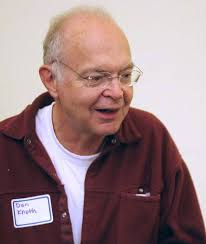
\includegraphics[width=.4\textwidth]{img/knuth.jpg}
	\caption{Donald Knuth}
	\label{fig:knuth}
\end{figure}


\begin{figure}[!htb]
	\centering
	\includegraphics[width=.4\textwidth]{img/783px-Test-Logo.svg}
	\caption{Test}
	\label{fig:test}
\end{figure}

Abbildungen bindet man mit \verb=\includegraphics= in einer Umgebung
\verb=figure= ein.
Man kann dann im Text auf die Abbildung \ref{fig:knuth} verweisen.
Man muss beachten, dass die Abbildung in einer sogenannten
\enquote{fließenden} Umgebung eingebunden wird, d.h. beim Setzen des
Dokuments bestimmt \TeX, an welcher Stelle genau im Dokument die
Abbildung erscheint.

Wie man an diesem Beispiel sieht, kann man beliebige Abbildungen etwa
\verb=jpg= wie in diesem Beispiel, aber auch \verb=pdf= einbinden. Man
kann also Abbildungen mit einem Grafikprogramm erstellen, als
\verb=pdf= speichern und dann einbinden.

\newcommand{\tikz}{Ti\emph{k}Z}

Es gibt aber auch \tikz\ (= \tikz\ ist kein Zeichenprogramm), das der
deutsche Informatiker Till Tantau entwickelt hat. Damit ist es möglich,
Abbildungen zu \enquote{programmieren}. Die Projektseite von \tikz\ ist
\url{https://sourceforge.net/projects/pgf/}. Interessant sind auch
die Beispiele auf \url{http://www.texample.net/tikz/examples/}.

\section{Tabellen}

Tabellen werden in einer \enquote{fließenden} Umgebung namens
\verb=table= eingegeben. Der eigentliche Inhalt der Tabelle kommt in die
Umgebung \verb=tabular=.

\begin{table}[!htb]
	\centering
	\caption{Die Geschichte von \TeX\ und \LaTeX}
	\begin{tabular}{ r p{13cm}}
		\toprule
		Jahr & Entwicklung\\
		\midrule
		1977 & Donald Knuth beginnt mit der Entwicklung von \TeX.\\
		1985 & \LaTeX\ (mächtige Makros, die die Verwendung von \TeX\
			vereinfachen, in dem sie Struktur und Layout trennen) wird von
			Leslie Lamport in der Version 2.09 freigegeben.\\
		1986 & Feier der Fertigstellung von \TeX\ im Computer Museum in
		Boston\\
		1986 & Leslie Lamport veröffentlicht \emph{\LaTeX: A Document
			Preparation System}.\\
		1993 & \LaTeXe\\
		2000 & pdf\TeX\ (entwickelt von Hàn Thé Thành)\\
			?  & Nach dem Tod von Donald Knuth bekommt \TeX\ die Versionsnummer
			$\pi$.\\
		\bottomrule
	\end{tabular}
	\label{tbl:geschichte}
\end{table}

Wie man am Beispiel des \LaTeX-Texts der Tabelle  \ref{tbl:geschichte}
sieht, kann die Formatierung von Tabellen etwas \enquote{sperrig} sein.
Gut, dass man sich in einer der vielen Anleitungen dazu erkundigen kann,
z.B. in der \LaTeXe-Kurzbeschreibung \cite[S.23]{lkurz15}.

\section{Listings}

\verb=listings= ist ein Paket, das es erlaubt, Code-Beispiele in die
Abschlussarbeit zu setzen. Wie das Beispiel \ref{lst:datei} zeigt, kann
man auch externe Dateien einbinden und im Text verbatim einsetzen. In
diesem Fall kann der eingebundene Text auch in der Zeichenkodierung
\emph{utf8} sein, wohingegen dies bei direkt im Text geschriebenen
Codebeispielen nicht unterstützt wird.

\begin{lstlisting}[caption={Einbinden einer Quelldatei}\label{lst:datei}]
% Der Inhalt der Datei myclass.java wird verbatim hier eingefügt
\lstinputlisting[caption={Eine Java-Klasse}\label{lst:java}]{myclass.java}
\end{lstlisting}

Für Listings gibt es viele Optionen des Layouts, insbesondere ist es
möglich die Programmiersprache des eingebundenen Code-Beispiels
anzugeben, was dazu führt, dass Schlüsselworte, Bezeichner und Kommentare
der Sprache im Layout hervorgehoben werden.

\section{Mathematische Formeln}

Mathematisches kann man in den laufenden Text einbauen, wie etwa bei
folgender Definition:

Mit $k!$, der Fakultät einer natürlichen Zahl $k$ bezeichnet man das
Produkt $1 \cdot 2 \cdot \dotso \cdot k$.

Oft braucht man aber auch ganze Abschnitte im Mathematik-Modus, wie in
folgendem Beispiel:

		Die sogenannte Collatz-Folge\footnote{ nach Lothar Collatz,
		deutscher Mathematiker 1910 - 1990} zu einer natürlichen Zahl $n$
		wird folgendermaßen gebildet:

	\begin{align}
	  n_1 &= n \nonumber \\
		n_{i+1} &= \left\{ \begin{array}{l l}
	                   n_i/2      & \textrm{falls $n_i$ gerade}\\
										 3 n_i + 1  & \textrm{falls $n_i$ ungerade}
										 \end{array} \right. \nonumber
	\end{align}

	\medskip
										 
	Startet man etwa mit der Zahl $7$ erhält man

	\[7\ 22\ 11\ 34\ 17\ 52\ 26\ 13\ 40\ 20\ 10\ 5\ 16\ 8\ 4\ 2\ 1\ 4\ 2\ 1\ \dots\]

	Wie man sieht, geht die Folge schließlich in den Zyklus $1, 4, 2$
	über.  Die \emph{Collatz-Vermutung} besagt, dass dies für jeden
	Startwert $n$ der Fall ist, d.h.  jede Collatz-Folge erreicht
	irgendwann den Wert $1$.

Mehr über das Setzen von mathematischen Formeln steht in \cite[Kapitel 4]{lkurz15}.



% ----------------------------------------------------------------------------
    % Kapitel 3

\end{lstlisting}

% ----------------------------------------------------------------------------
      % Kapitel 1
% ----------------------------------------------------------------------------
% Copyright (c) 2016 -2020 by Burkhardt Renz. All rights reserved.
% Die Vorlage für eine Abschlussarbeit in der Informatik am Fachbereich
% MNI der THM ist lizenziert unter einer Creative Commons
% Namensnennung-Nicht kommerziell 4.0 International Lizenz.
%
% Id:$
% ----------------------------------------------------------------------------

\chapter{Elemente für die Gliederung}

Der Text dieses Kapitels steht in \verb=gliederung.tex=. Er bezieht sich
auf \verb=vorlage.tex= und \verb=gliederung.tex=.

\section{Teile}

Eine Abschlussarbeit besteht aus drei großen Teilen:

\begin{itemize}
	\item Dem Vorderteil (\verb=frontmatter=) mit
		\begin{itemize}
			\item der Titelseite,
			\item der eidesstattlichen Erklärung,
			\item der Zusammenfassung,
			\item dem Inhaltsverzeichnis und
			\item den Verzeichnissen von Abbildungen, Tabellen und Listings,
		\end{itemize}
	\item dem Hauptteil (\verb=mainmatter=) mit den Kapiteln der Arbeit
		und
	\item dem Anhang (\verb=backmatter=) mit Anhängen und dem
		Literaturverzeichnis	
\end{itemize}

Manchmal erwarten Dozentinnen oder Dozenten, dass eine Abschlussarbeit
Verzeichnisse der Abbildungen, Tabellen und Listings oder auch ein Glossar
der verwendeten Begriffe enthält. Deshalb enthält unsere Vorlage diese
Verzeichnisse. Ein Glossar kann man mit der Umgebung \verb=description=
oder \verb=labeling= erzeugen, die in Abschnitt
\ref{sec:stichwortlisten}  beschrieben werden.

Ich persönlich finde, dass man auf diese Verzeichnisse verzichten kann.
Und ein Glossar ist meines Erachtens nur nötig, wenn man viele
Fachbegriffe in der Arbeit verwendet, die einem in der Informatik
Kundigen nicht geläufig sind.

\section{Kapitel und ihre Untergliederungen}

Die Dokumentklasse \verb=scrbook= hat als Möglichkeiten der Gliederung
zunächst den Teil (\verb=part=). Er wird in diesem Dokument nicht
verwendet und meistens ist eine Bachelor- oder Masterarbeit nicht so
umfangreich, als dass man sie in Teile unterteilen müsste.

Die nächste Ebene ist das Kapital (\verb=chapter=), wie wir auf der
vorigen Seite den Anfang eines solchen sehen. Kapitel beginnen immer auf
einer rechten Seite.

Dann kommt der Abschnitt (\verb=section=) --- in einem solchen befinden wir
uns im Moment.

\subsection{Unterabschnitt}

Dies ist eine \verb=subsection=.

\subsubsection{Unterunterabschnitt}

Jetzt sind wir noch eine Ebene tiefer, in der \verb=subsubsection=. Eine
Gliederung sollte ausgewogen sein, auch in Bezug auf die
Gliederungstiefe. Deshalb sollte man eher nicht bis zum
Unterunterabschnitt gehen.


\paragraph{Absatz mit Überschrift}

Dies ist ein Absatz mit Überschrift \verb=paragraph=. Die Überschrift
wird im Dokument hervorgehoben, hat aber keine eigene Zeile. Typografen
nennen das auch einen \enquote{Spieß}.

\subparagraph{Unterabsatz}

Dies ist ein Unterabsatz \verb=subparagraph=, auch ein \enquote{Spieß}.

\section{Untergliederungen im Text}

\subsection{Aufzählungen}

Man kann nummerierte Aufzählungen mit der Umgebung \verb=enumerate=
erzeugen. Dies eignet sich für Aufzählungen, die eine Reihenfolge haben
und ist oft einer Aneinanderreihung im Text vorzuziehen, weil
übersichtlicher.

Eine Bachelorarbeit besteht aus

\begin{enumerate}
	\item einem ersten Kapitel
		\begin{enumerate}
			\item einem ersten Abschnitt darin,
			\item einem zweiten Abschnitt darin,
		\end{enumerate}
	\item einem zweiten Kapitel
	\item usw. usf.	
\end{enumerate}

Aufzählungen, die keine inhaltliche Reihenfolge haben, kann man mit der
Umgebung \verb=itemize= darstellen:

\begin{itemize}
	\item eine wichtige Aussage
	\item noch eine wichtige Aussage
		\begin{itemize}
			\item mit einer Ausprägung
			\item und noch einer Ausprägung	
		\end{itemize}
	\item \dots
\end{itemize}

\subsection{Stichwortlisten}
\label{sec:stichwortlisten}

Ein Beispiel für die Umgebung \verb=description= habe ich aus der
Dokumentation von \textsf{KOMA-Script} übernommen:

\begin{description}
	\item[empty] ist der Seitenstil, bei dem Kopf- und Fußzeile vollständig 
		leer bleiben. 
	\item[plain] ist der Seitenstil, bei dem keinerlei Kolumnentitel verwendet wird. 
	\item[headings] ist der Seitenstil für automatische Kolumnentitel. 
	\item[myheadings] ist der Seitenstil für manuelle Kolumnentitel. 
\end{description}

Es gibt auch noch die Umgebung \verb=labeling=, bei der man durch ein
Muster angeben kann, wie breit die Einrückung ist. Im Beispiel mit den
Seitenstilen könnte man das so machen:

\setkomafont{labelinglabel}{\sffamily\bfseries}
\begin{labeling}{myheadings}
	\item[empty] ist der Seitenstil, bei dem Kopf- und Fußzeile vollständig 
		leer bleiben. 
	\item[plain] ist der Seitenstil, bei dem keinerlei Kolumnentitel verwendet wird. 
	\item[headings] ist der Seitenstil für automatische Kolumnentitel. 
	\item[myheadings] ist der Seitenstil für manuelle Kolumnentitel. 
\end{labeling}

\section{Zum Literaturverzeichnis}

In der Vorlage findet man das Literaturverzeichnis in der Datei
\verb=litverz.tex=. 

Das Literaturverzeichnis kann man in \LaTeX\ auf zwei Arten erstellen:

Die einfache Variante besteht darin, dass man die Umgebung
\verb=bibliography= verwendet. So haben wir das in diesem Dokument
gemacht. Die Angaben zur Literatur stehen in \verb=litverz=. Jeder
Eintrag hat einen \emph{key}, den wir im Text im Befehl \verb=\cite=
referenzieren können. Die Referenz wird dann als Nummer im Text
angegeben und die entsprechende Nummer erscheint auch im
Literaturverzeichnis.

Die etwas aufwändigere Variante besteht darin, \verb=bibtex= zu
verwenden. Dies lohnt sich insbesondere dann, wenn man in verschiedenen
Manuskripte immer wieder dieselben Literaturverweise verwendet.

Mit \verb=bibtex= speichert man die Literaturangaben in einer Art
Datenbank, einer BibTeX-Datei. Die im Manuskript referenzierten Arbeiten
werden dann von \verb=bibtex= automatisch in das Literaturverzeichnis
übernommen. Die Formatierung des Verweises im Text und der Einträge im
Literaturverzeichnis wird dabei durch eine eigene Datei, dem
BibTeX-Stil, gesteuert. Will man die Verweise durch Nummern, wählt man
als Stil \verb=plain=, will man die Verweise durch die Abkürzung des
Autorennamens mit Angabe des Jahres, wählt man z.B. den Stil
\verb=alpha=. Es gibt eine Vielzahl solcher BibTeX-Stile, siehe
\url{https://www.ctan.org/tex-archive/biblio/bibtex/contrib}. Man kann sogar
eigene BibTeX-Stile definieren mit \verb=tex makebst=.

Mehr über BibTeX findet man z.B. bei \url{https://de.wikibooks.org/wiki/LaTeX-Kompendium:_Zitieren_mit_BibTeX}.

% ----------------------------------------------------------------------------
  % Kapitel 2
% ----------------------------------------------------------------------------
% Copyright (c) 2016 - 2020 by Burkhardt Renz. All rights reserved.
% Die Vorlage für eine Abschlussarbeit in der Informatik am Fachbereich
% MNI der THM ist lizenziert unter einer Creative Commons
% Namensnennung-Nicht kommerziell 4.0 International Lizenz.
%
% Id:$
% ----------------------------------------------------------------------------

\chapter{Elemente im Text}

Der Text dieses Kapitels steht in \verb=elemente.tex= und bezieht auch
auf diese Datei.

\section{Typografische Elemente}

Im laufenden Text kann man alles Mögliche machen. Gute Typografie geht
mit diesen Möglichkeiten sparsam um. Was in Texten der Informatik oft
vorkommt ist die \emph{Hervorhebung} mit dem Befehl \verb=\emph=. Man
verwendet kursive Schrift auch für fremdsprachige Worte im Text, etwa
\textit{digital typography}.
Für Schlüsselworte, Befehle der Kommandozeile u.ä. nimmt man gerne einen
passenden Zeichensatz, etwa \texttt{make vorlage.pdf}. 

Das Paket \verb=csquotes= sorgt dafür dass Anführungszeichen
typografisch korrekt verwendet werden. Im Deutschen werden die
\enquote{Gänsefüßchen} nämlich anders als die angelsächsischen
\foreignquote{english}{quotation marks} gesetzt.

Mehr über das Setzen von Text findet man in \cite{lkurz15}.

\section{Referenzen und Links}

Verweise auf die Literatur macht man mit dem Befehl \verb=\cite=.
Braucht man Querverweise auf Abschnitte im Text oder Abbildungen etc.,
so versieht man das Verweisziel mit einem \verb=\label= und verweist
dann mit \verb=\ref= oder \verb=\pageref=. Mehr dazu in
\cite[S.50]{partosch15}.

Links auf Quellen im Internet werden durch den Befehl \verb=\url=
angegeben und dadurch in PDF \enquote{anklickbar}, etwa wie
\url{https://tug.org/mactex/src/WelcomeToMacTeX.pdf}.

\section{Abbildungen}

\begin{figure}[!htb]
	\centering
	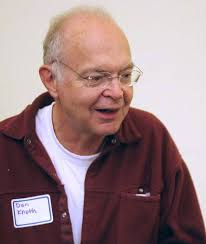
\includegraphics[width=.4\textwidth]{img/knuth.jpg}
	\caption{Donald Knuth}
	\label{fig:knuth}
\end{figure}


\begin{figure}[!htb]
	\centering
	\includegraphics[width=.4\textwidth]{img/783px-Test-Logo.svg}
	\caption{Test}
	\label{fig:test}
\end{figure}

Abbildungen bindet man mit \verb=\includegraphics= in einer Umgebung
\verb=figure= ein.
Man kann dann im Text auf die Abbildung \ref{fig:knuth} verweisen.
Man muss beachten, dass die Abbildung in einer sogenannten
\enquote{fließenden} Umgebung eingebunden wird, d.h. beim Setzen des
Dokuments bestimmt \TeX, an welcher Stelle genau im Dokument die
Abbildung erscheint.

Wie man an diesem Beispiel sieht, kann man beliebige Abbildungen etwa
\verb=jpg= wie in diesem Beispiel, aber auch \verb=pdf= einbinden. Man
kann also Abbildungen mit einem Grafikprogramm erstellen, als
\verb=pdf= speichern und dann einbinden.

\newcommand{\tikz}{Ti\emph{k}Z}

Es gibt aber auch \tikz\ (= \tikz\ ist kein Zeichenprogramm), das der
deutsche Informatiker Till Tantau entwickelt hat. Damit ist es möglich,
Abbildungen zu \enquote{programmieren}. Die Projektseite von \tikz\ ist
\url{https://sourceforge.net/projects/pgf/}. Interessant sind auch
die Beispiele auf \url{http://www.texample.net/tikz/examples/}.

\section{Tabellen}

Tabellen werden in einer \enquote{fließenden} Umgebung namens
\verb=table= eingegeben. Der eigentliche Inhalt der Tabelle kommt in die
Umgebung \verb=tabular=.

\begin{table}[!htb]
	\centering
	\caption{Die Geschichte von \TeX\ und \LaTeX}
	\begin{tabular}{ r p{13cm}}
		\toprule
		Jahr & Entwicklung\\
		\midrule
		1977 & Donald Knuth beginnt mit der Entwicklung von \TeX.\\
		1985 & \LaTeX\ (mächtige Makros, die die Verwendung von \TeX\
			vereinfachen, in dem sie Struktur und Layout trennen) wird von
			Leslie Lamport in der Version 2.09 freigegeben.\\
		1986 & Feier der Fertigstellung von \TeX\ im Computer Museum in
		Boston\\
		1986 & Leslie Lamport veröffentlicht \emph{\LaTeX: A Document
			Preparation System}.\\
		1993 & \LaTeXe\\
		2000 & pdf\TeX\ (entwickelt von Hàn Thé Thành)\\
			?  & Nach dem Tod von Donald Knuth bekommt \TeX\ die Versionsnummer
			$\pi$.\\
		\bottomrule
	\end{tabular}
	\label{tbl:geschichte}
\end{table}

Wie man am Beispiel des \LaTeX-Texts der Tabelle  \ref{tbl:geschichte}
sieht, kann die Formatierung von Tabellen etwas \enquote{sperrig} sein.
Gut, dass man sich in einer der vielen Anleitungen dazu erkundigen kann,
z.B. in der \LaTeXe-Kurzbeschreibung \cite[S.23]{lkurz15}.

\section{Listings}

\verb=listings= ist ein Paket, das es erlaubt, Code-Beispiele in die
Abschlussarbeit zu setzen. Wie das Beispiel \ref{lst:datei} zeigt, kann
man auch externe Dateien einbinden und im Text verbatim einsetzen. In
diesem Fall kann der eingebundene Text auch in der Zeichenkodierung
\emph{utf8} sein, wohingegen dies bei direkt im Text geschriebenen
Codebeispielen nicht unterstützt wird.

\begin{lstlisting}[caption={Einbinden einer Quelldatei}\label{lst:datei}]
% Der Inhalt der Datei myclass.java wird verbatim hier eingefügt
\lstinputlisting[caption={Eine Java-Klasse}\label{lst:java}]{myclass.java}
\end{lstlisting}

Für Listings gibt es viele Optionen des Layouts, insbesondere ist es
möglich die Programmiersprache des eingebundenen Code-Beispiels
anzugeben, was dazu führt, dass Schlüsselworte, Bezeichner und Kommentare
der Sprache im Layout hervorgehoben werden.

\section{Mathematische Formeln}

Mathematisches kann man in den laufenden Text einbauen, wie etwa bei
folgender Definition:

Mit $k!$, der Fakultät einer natürlichen Zahl $k$ bezeichnet man das
Produkt $1 \cdot 2 \cdot \dotso \cdot k$.

Oft braucht man aber auch ganze Abschnitte im Mathematik-Modus, wie in
folgendem Beispiel:

		Die sogenannte Collatz-Folge\footnote{ nach Lothar Collatz,
		deutscher Mathematiker 1910 - 1990} zu einer natürlichen Zahl $n$
		wird folgendermaßen gebildet:

	\begin{align}
	  n_1 &= n \nonumber \\
		n_{i+1} &= \left\{ \begin{array}{l l}
	                   n_i/2      & \textrm{falls $n_i$ gerade}\\
										 3 n_i + 1  & \textrm{falls $n_i$ ungerade}
										 \end{array} \right. \nonumber
	\end{align}

	\medskip
										 
	Startet man etwa mit der Zahl $7$ erhält man

	\[7\ 22\ 11\ 34\ 17\ 52\ 26\ 13\ 40\ 20\ 10\ 5\ 16\ 8\ 4\ 2\ 1\ 4\ 2\ 1\ \dots\]

	Wie man sieht, geht die Folge schließlich in den Zyklus $1, 4, 2$
	über.  Die \emph{Collatz-Vermutung} besagt, dass dies für jeden
	Startwert $n$ der Fall ist, d.h.  jede Collatz-Folge erreicht
	irgendwann den Wert $1$.

Mehr über das Setzen von mathematischen Formeln steht in \cite[Kapitel 4]{lkurz15}.



% ----------------------------------------------------------------------------
    % Kapitel 3

\end{lstlisting}

% ----------------------------------------------------------------------------
      % Kapitel 1
% ----------------------------------------------------------------------------
% Copyright (c) 2016 -2020 by Burkhardt Renz. All rights reserved.
% Die Vorlage für eine Abschlussarbeit in der Informatik am Fachbereich
% MNI der THM ist lizenziert unter einer Creative Commons
% Namensnennung-Nicht kommerziell 4.0 International Lizenz.
%
% Id:$
% ----------------------------------------------------------------------------

\chapter{Elemente für die Gliederung}

Der Text dieses Kapitels steht in \verb=gliederung.tex=. Er bezieht sich
auf \verb=vorlage.tex= und \verb=gliederung.tex=.

\section{Teile}

Eine Abschlussarbeit besteht aus drei großen Teilen:

\begin{itemize}
	\item Dem Vorderteil (\verb=frontmatter=) mit
		\begin{itemize}
			\item der Titelseite,
			\item der eidesstattlichen Erklärung,
			\item der Zusammenfassung,
			\item dem Inhaltsverzeichnis und
			\item den Verzeichnissen von Abbildungen, Tabellen und Listings,
		\end{itemize}
	\item dem Hauptteil (\verb=mainmatter=) mit den Kapiteln der Arbeit
		und
	\item dem Anhang (\verb=backmatter=) mit Anhängen und dem
		Literaturverzeichnis	
\end{itemize}

Manchmal erwarten Dozentinnen oder Dozenten, dass eine Abschlussarbeit
Verzeichnisse der Abbildungen, Tabellen und Listings oder auch ein Glossar
der verwendeten Begriffe enthält. Deshalb enthält unsere Vorlage diese
Verzeichnisse. Ein Glossar kann man mit der Umgebung \verb=description=
oder \verb=labeling= erzeugen, die in Abschnitt
\ref{sec:stichwortlisten}  beschrieben werden.

Ich persönlich finde, dass man auf diese Verzeichnisse verzichten kann.
Und ein Glossar ist meines Erachtens nur nötig, wenn man viele
Fachbegriffe in der Arbeit verwendet, die einem in der Informatik
Kundigen nicht geläufig sind.

\section{Kapitel und ihre Untergliederungen}

Die Dokumentklasse \verb=scrbook= hat als Möglichkeiten der Gliederung
zunächst den Teil (\verb=part=). Er wird in diesem Dokument nicht
verwendet und meistens ist eine Bachelor- oder Masterarbeit nicht so
umfangreich, als dass man sie in Teile unterteilen müsste.

Die nächste Ebene ist das Kapital (\verb=chapter=), wie wir auf der
vorigen Seite den Anfang eines solchen sehen. Kapitel beginnen immer auf
einer rechten Seite.

Dann kommt der Abschnitt (\verb=section=) --- in einem solchen befinden wir
uns im Moment.

\subsection{Unterabschnitt}

Dies ist eine \verb=subsection=.

\subsubsection{Unterunterabschnitt}

Jetzt sind wir noch eine Ebene tiefer, in der \verb=subsubsection=. Eine
Gliederung sollte ausgewogen sein, auch in Bezug auf die
Gliederungstiefe. Deshalb sollte man eher nicht bis zum
Unterunterabschnitt gehen.


\paragraph{Absatz mit Überschrift}

Dies ist ein Absatz mit Überschrift \verb=paragraph=. Die Überschrift
wird im Dokument hervorgehoben, hat aber keine eigene Zeile. Typografen
nennen das auch einen \enquote{Spieß}.

\subparagraph{Unterabsatz}

Dies ist ein Unterabsatz \verb=subparagraph=, auch ein \enquote{Spieß}.

\section{Untergliederungen im Text}

\subsection{Aufzählungen}

Man kann nummerierte Aufzählungen mit der Umgebung \verb=enumerate=
erzeugen. Dies eignet sich für Aufzählungen, die eine Reihenfolge haben
und ist oft einer Aneinanderreihung im Text vorzuziehen, weil
übersichtlicher.

Eine Bachelorarbeit besteht aus

\begin{enumerate}
	\item einem ersten Kapitel
		\begin{enumerate}
			\item einem ersten Abschnitt darin,
			\item einem zweiten Abschnitt darin,
		\end{enumerate}
	\item einem zweiten Kapitel
	\item usw. usf.	
\end{enumerate}

Aufzählungen, die keine inhaltliche Reihenfolge haben, kann man mit der
Umgebung \verb=itemize= darstellen:

\begin{itemize}
	\item eine wichtige Aussage
	\item noch eine wichtige Aussage
		\begin{itemize}
			\item mit einer Ausprägung
			\item und noch einer Ausprägung	
		\end{itemize}
	\item \dots
\end{itemize}

\subsection{Stichwortlisten}
\label{sec:stichwortlisten}

Ein Beispiel für die Umgebung \verb=description= habe ich aus der
Dokumentation von \textsf{KOMA-Script} übernommen:

\begin{description}
	\item[empty] ist der Seitenstil, bei dem Kopf- und Fußzeile vollständig 
		leer bleiben. 
	\item[plain] ist der Seitenstil, bei dem keinerlei Kolumnentitel verwendet wird. 
	\item[headings] ist der Seitenstil für automatische Kolumnentitel. 
	\item[myheadings] ist der Seitenstil für manuelle Kolumnentitel. 
\end{description}

Es gibt auch noch die Umgebung \verb=labeling=, bei der man durch ein
Muster angeben kann, wie breit die Einrückung ist. Im Beispiel mit den
Seitenstilen könnte man das so machen:

\setkomafont{labelinglabel}{\sffamily\bfseries}
\begin{labeling}{myheadings}
	\item[empty] ist der Seitenstil, bei dem Kopf- und Fußzeile vollständig 
		leer bleiben. 
	\item[plain] ist der Seitenstil, bei dem keinerlei Kolumnentitel verwendet wird. 
	\item[headings] ist der Seitenstil für automatische Kolumnentitel. 
	\item[myheadings] ist der Seitenstil für manuelle Kolumnentitel. 
\end{labeling}

\section{Zum Literaturverzeichnis}

In der Vorlage findet man das Literaturverzeichnis in der Datei
\verb=litverz.tex=. 

Das Literaturverzeichnis kann man in \LaTeX\ auf zwei Arten erstellen:

Die einfache Variante besteht darin, dass man die Umgebung
\verb=bibliography= verwendet. So haben wir das in diesem Dokument
gemacht. Die Angaben zur Literatur stehen in \verb=litverz=. Jeder
Eintrag hat einen \emph{key}, den wir im Text im Befehl \verb=\cite=
referenzieren können. Die Referenz wird dann als Nummer im Text
angegeben und die entsprechende Nummer erscheint auch im
Literaturverzeichnis.

Die etwas aufwändigere Variante besteht darin, \verb=bibtex= zu
verwenden. Dies lohnt sich insbesondere dann, wenn man in verschiedenen
Manuskripte immer wieder dieselben Literaturverweise verwendet.

Mit \verb=bibtex= speichert man die Literaturangaben in einer Art
Datenbank, einer BibTeX-Datei. Die im Manuskript referenzierten Arbeiten
werden dann von \verb=bibtex= automatisch in das Literaturverzeichnis
übernommen. Die Formatierung des Verweises im Text und der Einträge im
Literaturverzeichnis wird dabei durch eine eigene Datei, dem
BibTeX-Stil, gesteuert. Will man die Verweise durch Nummern, wählt man
als Stil \verb=plain=, will man die Verweise durch die Abkürzung des
Autorennamens mit Angabe des Jahres, wählt man z.B. den Stil
\verb=alpha=. Es gibt eine Vielzahl solcher BibTeX-Stile, siehe
\url{https://www.ctan.org/tex-archive/biblio/bibtex/contrib}. Man kann sogar
eigene BibTeX-Stile definieren mit \verb=tex makebst=.

Mehr über BibTeX findet man z.B. bei \url{https://de.wikibooks.org/wiki/LaTeX-Kompendium:_Zitieren_mit_BibTeX}.

% ----------------------------------------------------------------------------
  % Kapitel 2
% ----------------------------------------------------------------------------
% Copyright (c) 2016 - 2020 by Burkhardt Renz. All rights reserved.
% Die Vorlage für eine Abschlussarbeit in der Informatik am Fachbereich
% MNI der THM ist lizenziert unter einer Creative Commons
% Namensnennung-Nicht kommerziell 4.0 International Lizenz.
%
% Id:$
% ----------------------------------------------------------------------------

\chapter{Elemente im Text}

Der Text dieses Kapitels steht in \verb=elemente.tex= und bezieht auch
auf diese Datei.

\section{Typografische Elemente}

Im laufenden Text kann man alles Mögliche machen. Gute Typografie geht
mit diesen Möglichkeiten sparsam um. Was in Texten der Informatik oft
vorkommt ist die \emph{Hervorhebung} mit dem Befehl \verb=\emph=. Man
verwendet kursive Schrift auch für fremdsprachige Worte im Text, etwa
\textit{digital typography}.
Für Schlüsselworte, Befehle der Kommandozeile u.ä. nimmt man gerne einen
passenden Zeichensatz, etwa \texttt{make vorlage.pdf}. 

Das Paket \verb=csquotes= sorgt dafür dass Anführungszeichen
typografisch korrekt verwendet werden. Im Deutschen werden die
\enquote{Gänsefüßchen} nämlich anders als die angelsächsischen
\foreignquote{english}{quotation marks} gesetzt.

Mehr über das Setzen von Text findet man in \cite{lkurz15}.

\section{Referenzen und Links}

Verweise auf die Literatur macht man mit dem Befehl \verb=\cite=.
Braucht man Querverweise auf Abschnitte im Text oder Abbildungen etc.,
so versieht man das Verweisziel mit einem \verb=\label= und verweist
dann mit \verb=\ref= oder \verb=\pageref=. Mehr dazu in
\cite[S.50]{partosch15}.

Links auf Quellen im Internet werden durch den Befehl \verb=\url=
angegeben und dadurch in PDF \enquote{anklickbar}, etwa wie
\url{https://tug.org/mactex/src/WelcomeToMacTeX.pdf}.

\section{Abbildungen}

\begin{figure}[!htb]
	\centering
	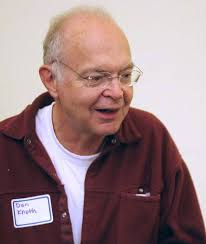
\includegraphics[width=.4\textwidth]{img/knuth.jpg}
	\caption{Donald Knuth}
	\label{fig:knuth}
\end{figure}


\begin{figure}[!htb]
	\centering
	\includegraphics[width=.4\textwidth]{img/783px-Test-Logo.svg}
	\caption{Test}
	\label{fig:test}
\end{figure}

Abbildungen bindet man mit \verb=\includegraphics= in einer Umgebung
\verb=figure= ein.
Man kann dann im Text auf die Abbildung \ref{fig:knuth} verweisen.
Man muss beachten, dass die Abbildung in einer sogenannten
\enquote{fließenden} Umgebung eingebunden wird, d.h. beim Setzen des
Dokuments bestimmt \TeX, an welcher Stelle genau im Dokument die
Abbildung erscheint.

Wie man an diesem Beispiel sieht, kann man beliebige Abbildungen etwa
\verb=jpg= wie in diesem Beispiel, aber auch \verb=pdf= einbinden. Man
kann also Abbildungen mit einem Grafikprogramm erstellen, als
\verb=pdf= speichern und dann einbinden.

\newcommand{\tikz}{Ti\emph{k}Z}

Es gibt aber auch \tikz\ (= \tikz\ ist kein Zeichenprogramm), das der
deutsche Informatiker Till Tantau entwickelt hat. Damit ist es möglich,
Abbildungen zu \enquote{programmieren}. Die Projektseite von \tikz\ ist
\url{https://sourceforge.net/projects/pgf/}. Interessant sind auch
die Beispiele auf \url{http://www.texample.net/tikz/examples/}.

\section{Tabellen}

Tabellen werden in einer \enquote{fließenden} Umgebung namens
\verb=table= eingegeben. Der eigentliche Inhalt der Tabelle kommt in die
Umgebung \verb=tabular=.

\begin{table}[!htb]
	\centering
	\caption{Die Geschichte von \TeX\ und \LaTeX}
	\begin{tabular}{ r p{13cm}}
		\toprule
		Jahr & Entwicklung\\
		\midrule
		1977 & Donald Knuth beginnt mit der Entwicklung von \TeX.\\
		1985 & \LaTeX\ (mächtige Makros, die die Verwendung von \TeX\
			vereinfachen, in dem sie Struktur und Layout trennen) wird von
			Leslie Lamport in der Version 2.09 freigegeben.\\
		1986 & Feier der Fertigstellung von \TeX\ im Computer Museum in
		Boston\\
		1986 & Leslie Lamport veröffentlicht \emph{\LaTeX: A Document
			Preparation System}.\\
		1993 & \LaTeXe\\
		2000 & pdf\TeX\ (entwickelt von Hàn Thé Thành)\\
			?  & Nach dem Tod von Donald Knuth bekommt \TeX\ die Versionsnummer
			$\pi$.\\
		\bottomrule
	\end{tabular}
	\label{tbl:geschichte}
\end{table}

Wie man am Beispiel des \LaTeX-Texts der Tabelle  \ref{tbl:geschichte}
sieht, kann die Formatierung von Tabellen etwas \enquote{sperrig} sein.
Gut, dass man sich in einer der vielen Anleitungen dazu erkundigen kann,
z.B. in der \LaTeXe-Kurzbeschreibung \cite[S.23]{lkurz15}.

\section{Listings}

\verb=listings= ist ein Paket, das es erlaubt, Code-Beispiele in die
Abschlussarbeit zu setzen. Wie das Beispiel \ref{lst:datei} zeigt, kann
man auch externe Dateien einbinden und im Text verbatim einsetzen. In
diesem Fall kann der eingebundene Text auch in der Zeichenkodierung
\emph{utf8} sein, wohingegen dies bei direkt im Text geschriebenen
Codebeispielen nicht unterstützt wird.

\begin{lstlisting}[caption={Einbinden einer Quelldatei}\label{lst:datei}]
% Der Inhalt der Datei myclass.java wird verbatim hier eingefügt
\lstinputlisting[caption={Eine Java-Klasse}\label{lst:java}]{myclass.java}
\end{lstlisting}

Für Listings gibt es viele Optionen des Layouts, insbesondere ist es
möglich die Programmiersprache des eingebundenen Code-Beispiels
anzugeben, was dazu führt, dass Schlüsselworte, Bezeichner und Kommentare
der Sprache im Layout hervorgehoben werden.

\section{Mathematische Formeln}

Mathematisches kann man in den laufenden Text einbauen, wie etwa bei
folgender Definition:

Mit $k!$, der Fakultät einer natürlichen Zahl $k$ bezeichnet man das
Produkt $1 \cdot 2 \cdot \dotso \cdot k$.

Oft braucht man aber auch ganze Abschnitte im Mathematik-Modus, wie in
folgendem Beispiel:

		Die sogenannte Collatz-Folge\footnote{ nach Lothar Collatz,
		deutscher Mathematiker 1910 - 1990} zu einer natürlichen Zahl $n$
		wird folgendermaßen gebildet:

	\begin{align}
	  n_1 &= n \nonumber \\
		n_{i+1} &= \left\{ \begin{array}{l l}
	                   n_i/2      & \textrm{falls $n_i$ gerade}\\
										 3 n_i + 1  & \textrm{falls $n_i$ ungerade}
										 \end{array} \right. \nonumber
	\end{align}

	\medskip
										 
	Startet man etwa mit der Zahl $7$ erhält man

	\[7\ 22\ 11\ 34\ 17\ 52\ 26\ 13\ 40\ 20\ 10\ 5\ 16\ 8\ 4\ 2\ 1\ 4\ 2\ 1\ \dots\]

	Wie man sieht, geht die Folge schließlich in den Zyklus $1, 4, 2$
	über.  Die \emph{Collatz-Vermutung} besagt, dass dies für jeden
	Startwert $n$ der Fall ist, d.h.  jede Collatz-Folge erreicht
	irgendwann den Wert $1$.

Mehr über das Setzen von mathematischen Formeln steht in \cite[Kapitel 4]{lkurz15}.



% ----------------------------------------------------------------------------
    % Kapitel 3

\end{lstlisting}

% ----------------------------------------------------------------------------
